\section{Methods}

In order to demonstrate that the DISHTINY platform selects for detectable hierarchical transitions in individuality, we performed experiments where cell-like organisms evolved parameters to control manually-designed strategies such as resource-sharing, reproductive decision-making, and apoptosis.
We will first cover the design of the DISHTINY platform and then describe the simple cell-like organisms we used to evaluate the platform.

\subsection{DISHTINY}

\begin{figure*}[t]
\begin{center}
\includegraphics[width=2.0\columnwidth]{img/explanatory}
\caption{
\textbf{Activation signaling, and net resource collection for three different-sized same-channel networks during a resource wave event.}
At the top, a resource wave is depicted propagating over three updates and then ceasing for four updates (left to right).
In row $a$, a small two-cell channel-signaling group (far left, in green) is activated; tracking the resource wave (top) yields a small net resource harvest (far right).
In row $b$, an intermediate-sized 13-cell channel-signaling group yields a high net resource harvest.
Finally, in row $c$, a large 29-cell channel-signaling group incurs a net negative resource harvest.
In rows $a$, $b$, and $c$, dark purple indicates the active state, light purple indicates the quiescent state, and white indicates the ready state.
}
\label{fig:explanatory}
\end{center}
\end{figure*}


DISHTINY allows cell-like organisms to replicate across a toroidal grid.
Over discrete timesteps (``updates''), the cells can collect a continuous-valued resource.
Once sufficient resource has been accrued, cells may pay $3.0$ resource to place a daughter cell on an adjoining tile of the toroidal grid (i.e., reproduce), replacing any existing cell already there.
As cells reproduce, they can choose to include offspring in the parent's cooperating ``signaling channel'' group or force offspring to create a new cooperating ``signaling channel'' group.

As shown at the top of Figure \ref{fig:explanatory}, resources appear at a single point then spread outwards update-by-update in a diamond-shaped wave, disappearing when the expanding wave reaches a predefined limit.
Cells must be in a costly ``activated'' state to collect resource as it passes.
The cell at the starting position of a resource wave is automatically activated, and will send the activate signal to neighboring cells on the same signaling channel.
The newly activated cells, in turn, activate their own neighbors registered to the same signaling channel.
Neighbors registered to other signaling channels do not activate.
Each cell, after sending the activation signal, enters a temporary quiescent state so as not to reactivate from the signal.
In this manner, cells sharing a signaling channel activate in concert with the expanding resource wave.
As shown Figure \ref{fig:explanatory}$a,b$, the rate of resource collection for a cell is determined by the size and shape of of its same-channel signaling network;
small or fragmented same-channel signaling networks will frequently miss out on resource as it passes by.

Each cell pays a resource cost when it activates.
This cost is outweighed by the resource collected such that cells that activate in concert with a resource wave derive a net benefit.
Recall, though, that resource waves have a limited extent.
Cells that activate outside the extent of a resource wave or activate out of sync with the resource wave (due to an indirect path from the cell that originated the signal) pay the activation cost but collect no resource.
Cells that frequently activate erroneously use up their resource and die.
In our implementation, organisms that accrue a resource debt of $-5$ or greater are killed.
This erroneous activation scenario is depicted in Figure \ref{fig:explanatory}$c$.

In this manner, ``Goldilocks'' --- not to small and not too big --- signaling networks are selected for.
Based on a randomly chosen starting location, resource wave starting points (seeds) are tiled over the toroidal grid such that the extents of the resource waves touch, but do not overlap.
All waves start and proceed synchronously;
when they complete, the next resource waves are seeded.
This process ensures that selection for ``Goldilocks'' same-channel signaling networks is uniformly distributed over the toroidal grid.

Cells control the size and shape of their same-channel signaling group through strategic reproduction.
Three choices are afforded: whether to reproduce at all, where among the four adjoining tiles of the toroidal grid to place their offspring, and whether the offspring should be registered to the parent's signaling channel or be given a random channel ID (in the range 1 to $2^{64}$).
The probability of channel collision is miniscule: $60 \times 60 \times 50100$ (the grid dimensions times the number of simulation updates) independent channel values will only collide with probability $1 \times 10^{-11}$.
No guarantees are made about the uniqueness of a newly-generated channel ID, but chance collisions are rare.

To ensure turnover of channel groups, a channel generation limit is enforced.
Each time a cell spawns a daughter cell sharing the same channel, the parent's channel generation counter is incremented and the daughter cell's channel generation counter is then initialized to match their  parent's counter.
Once the channel generation counter reaches a limit, in this implementation defined as the resource wave radius, daughter cells may no longer be endowed with the parent's channel ID; a new, randomly-drawn channel ID is assigned to daughter cells instead.

Hierarchical levels are introduced into the system through multiple separate, but overlaid, instantiations of this resource wave/channel-signaling scheme.
We refer to each independent resource wave/channel-signaling system as a ``level.''
In our experiments, we allowed two resource wave/channel-signaling levels, identified here as level one and level two.
On level one, resource waves extended a radius of three toroidal tiles.
On level two they extended a radius of 24 toroidal tiles.
On both levels, activated cells netted $+1.0$ resource from a resource wave, but suffered an activation penalty of $-5.0$ if no resource was available.
Due to the different radii of resource waves on different levels, level one selects for small same-channel signaling networks and level two selects for large same-channel signaling networks.

Cells were marked with two separate channel IDs, one for level one and another for level two.
We enforced hierarchical nesting of same-channel signaling networks during reproduction:
daughter cells may inherit neither channel ID, just the level-two channel ID, or both channel IDs.
Daughter cells may not inherit only the level-one channel ID while having a different level-two channel ID.
The distribution of IDs across the level-two and level-one channels can be envisioned by analogy to political countries and territories.
Each country (i.e., level-two channel network) may have one or many territories (i.e., level-one channel network).
However, no territory spans more than one country.
Figure \ref{fig:outcome_grids} depicts hierarchically nested channel states at the end of three evolutionary runs.

Channel IDs enable straightforward detection of an evolutionary transition in individuality.
Because common channel IDs may only arise systematically through inheritance, common channel IDs indicate a close hereditary relationship in addition to a close cooperative relationship.
Because new channel IDs arise first in a single cell, same-channel signaling networks are reproductively bottlenecked, ensuring meaningful reproductive lineages at the level of the same-channel signaling network.
To recognize an evolutionary transition in individuality, we therefore evaluate
\begin{enumerate}
\item Do cells with the same channel ID choose to share resources (e.g., cooperate)?
\item Is there division of reproductive labor between members of the same channel (e.g., do cells at the interior of a network cede reproduction to those at the periphery?)
\end{enumerate}
If these conditions are met among cells sharing the same level-one channel, a first-level transition in individuality may have occurred.
Likewise, if these conditions are met among cells sharing the same level-two channel, a second-level transition in individuality may have occurred.
In either case, observation of altruistic behavior, such as an apoptosis response to mutation, would further evidence a transition.

\subsection{Organisms}

\begin{figure*}[t]
\begin{center}
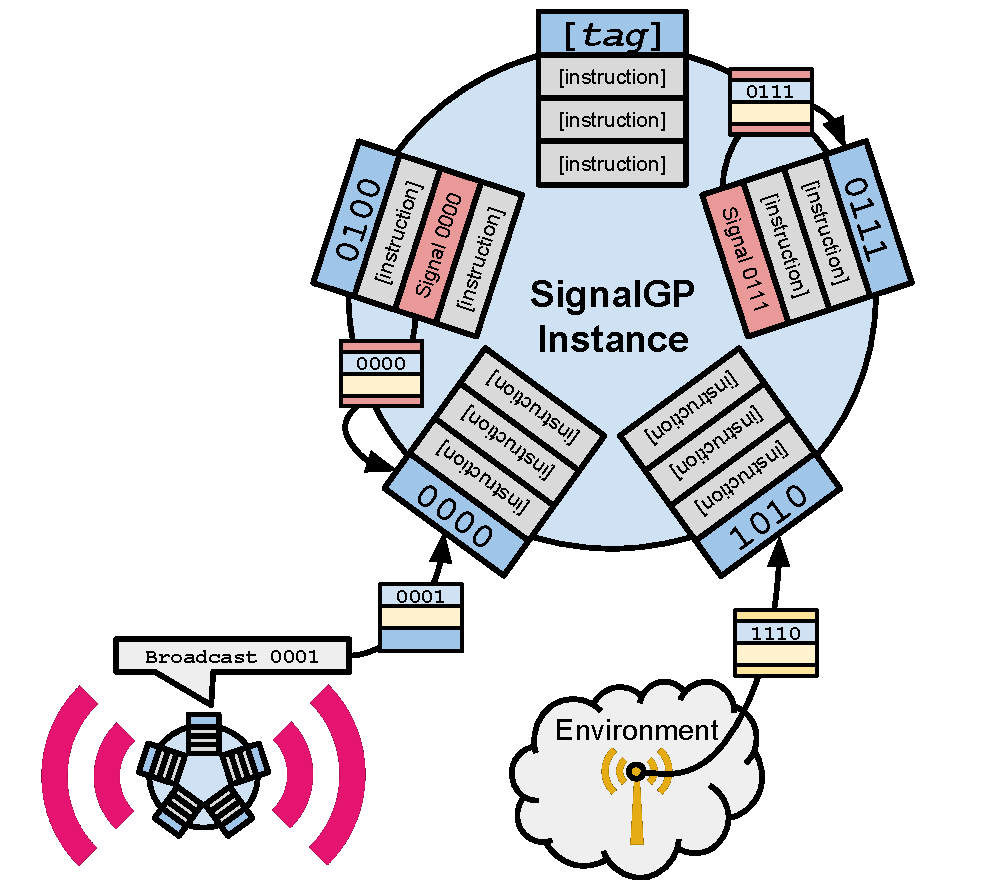
\includegraphics[width=\columnwidth]{img/signalgp-cartoon}%
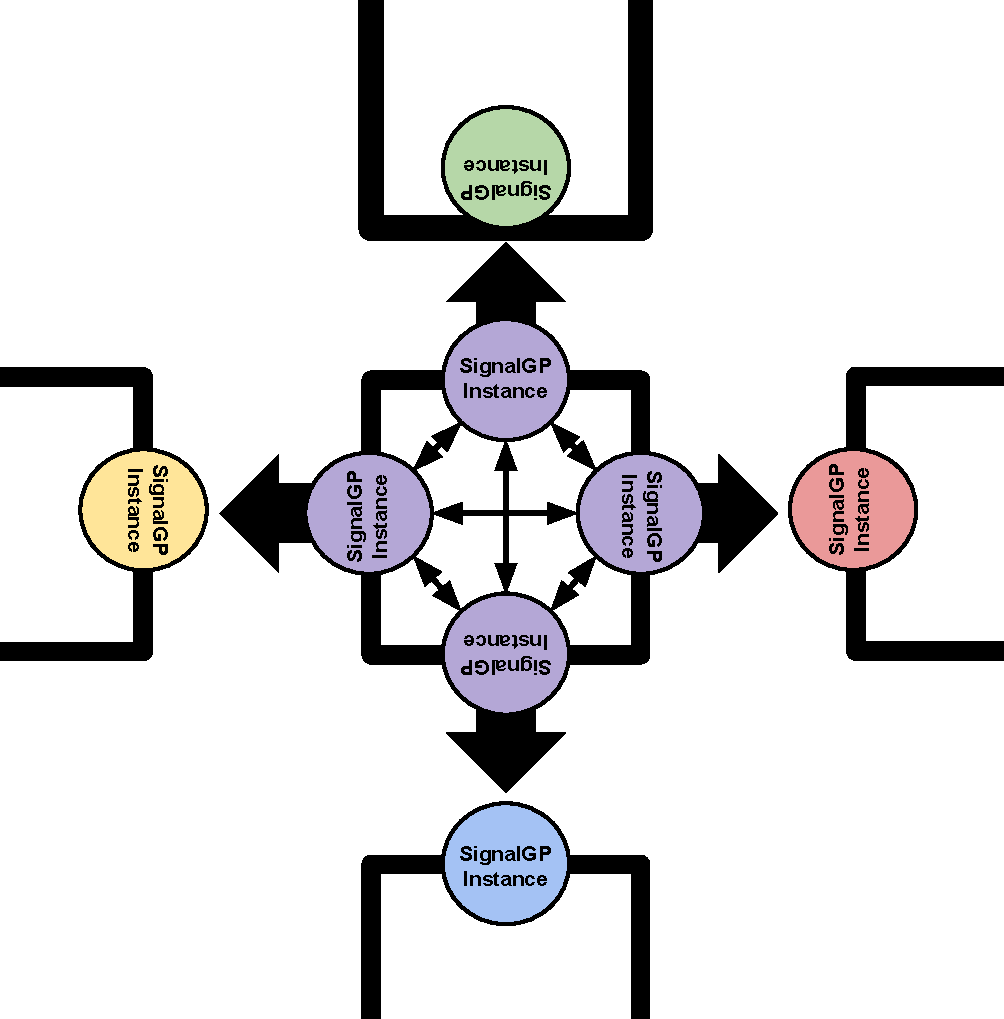
\includegraphics[width=\columnwidth]{img/dishtinygp-cartoon}
\caption{TODO}
\label{fig:signalgp-dishtinygp}
\end{center}
\end{figure*}


We performed our experiments using cell-level organisms based on SignalGP \cite{lalejini2018evolving}.
These cell-level organisms are in no way inherent to the DISHTINY platform, but were merely developed to study the platform.

In order to ensure symmetry
unlike previous work on grid-based cooperation

A combination of event-driven and procedural sensing.

\subsection{Instruction Library}

generic instructions in the default SignalGP instruction set \cite{lalejini2018evolving}.

\begin{itemize}
\item \textbf{RNG Draw} Draw a random value between 0.0 and 1.0 from onboard random number generator and store result in register.
\item \textbf{Send/Broadcast Intracellular Message}
\item \textbf{Set Stockpile Reserve} sharing only
\item \textbf{Pause Reproduction} instance facing PauseRepr-Lev PauseRepr
\item \textbf{Activate/Deactivate Intercellular Inbox} ActivateInbox; at cell birth, begins in the de-activated state
\item \textbf{Deactivate Intracellular Inbox}  DeactivateInbox
\item \textbf{Share Resource} large (0.5) and small (0.05) modulated by argument
\item \textbf{Accept/Decline Sharing} accept sharing on cell birth
\item \textbf{Send/Broadcast Intercellular Message}
\item \textbf{Reproduce} try (resource, pause reproduction), lev, channel age
\item \textbf{Increase Channel Age} defined per level
\item \textbf{Apoptosis} partial and complete
\item \textbf{Designate/Revoke Heir} apoptosis 80\% of repduction cost and own stockpile amount
\item \textbf{Query Own Stockpile}
\item \textbf{Query Own Channel Age} -Lev
\item \textbf{Query Is Neighbor Live}
\item \textbf{Query Is Neighbor Channel Occupied}
\item \textbf{Query Is Neighbor My Cellular Child}
\item \textbf{Query Is Neighbor My Cellular Parent}
\item \textbf{Query Does Neighbor's Channel ID Match Mine} defined per level
\item \textbf{Query Does Neighbor's Channel ID Descend From Mine} defined for top level e.g., is neighbor my propagule
\item \textbf{Query Does My Channel ID Descend From Neighbor's} defined for top level level e.g., am I neighbor's propagule
\item \textbf{Query Neighbor's Channel ID}
\item \textbf{Query Neighbor's Stockpile}
\end{itemize}


\subsection{Event Library}

\begin{itemize}
\item \textbf{On Update}
\item \textbf{Facing Cellular Child}
\item \textbf{Stockpile Debt} negative resource
\item \textbf{Neighbor's Channel ID Matches Mine} defined per level
\item \textbf{Neighbor's Channel ID Descends From Mine} top level
e.g., is neighbor my propagule
\end{itemize}

Instruction set

Signals

\subsection{Treatments}

Three experimental parameters:
\begin{enumerate}
\item hierarchy (and wave size)
\item resource distribution (wave vs even)
\item recognize/sense channels (as proxy for kin)
\end{enumerate}

We performed six treatments with these combinations of experimental parameters
\begin{enumerate}
\item treat=resource-even\_channelsense-no\_nlev-two
\item treat=resource-wave\_channelsense-no\_nlev-two
\item treat=resource-wave\_channelsense-yes\_nlev-onesmall
\item treat=resource-even\_channelsense-yes\_nlev-two
\item treat=resource-wave\_channelsense-yes\_nlev-onebig
\item treat=resource-wave\_channelsense-yes\_nlev-two
\end{enumerate}

\subsection{Implementation}

We implemented our experimental system using the Empirical library for scientific software development in C++, available at \url{https://github.com/devosoft/Empirical}.
The code used to perform and analyze our experiments, our figures, data from our experiments, and a live in-browser demo of our system is available via the Open Science Framework at \url{https://osf.io/g58xk/}.
